\section{Certificant l'aplicació amb FamilySearch}\label{section:certification}

    \paragraph{}
    Com s'havia comentat en la quarta secció d'aquesta memòria, en la que s'introduïa l'API de FamilySearch, per tal d'obtenir accés a les dades de producció cal certificar les aplicacions.

    El procés de certificació, pot ser vist com una validació de l'aplicació per part de l'organització FamilySearch, per assegurar que no es realitza cap operació que pugui afectar al rendiment de l'API, la integritat de les dades o la seguretat del sistema.

    En el cas de la nostra aplicació, el conjunt de passos a realitzar per tal de certificar l'aplicació web s'exposen a continuació:

    \begin{enumerate}
        \item Aplicar l'aplicació per certificació des de la secció `les meves aplicacions' del portal de desenvolupadors de FamilySearch.
        \item Completar, signar i retornar l'acord d'afiliació de producte, les regles de seguretat i la petició d'obtenció d'una clau d'accés a producció.
        \item Registrar l'aplicació a FamilySearch i monitorar el procés de certificació.
        \item L'aplicació serà avaluada de diferents formes segons els diferents certificats que es vulguin obtenir. Aquests certificats van relacionats amb les operacions que realitza l'aplicació contra l'API.
    \end{enumerate}


    \subsection{Certificat d'autentificació}

    \paragraph{}
    El primer certificat que l'aplicació desenvolupada requereix és el relacionat amb el procés d'identificació dels usuaris a l'API de FamilySearch.

    La llista de consideracions a tenir en compte per obtenir el certificat són:

    \begin{itemize}
        \item Cada usuari ha d'adquirir un token d'identificació propi per tal de llegir dades de l'arbre familiar de FamilySearch.
        \item Els tokens d'identificació han de ser protegits. En cas que es vulgui emmagatzemar un token en una galeta del navegador, aquesta ha de ser una galeta segura.
        \item El tràfic és xifrat mitjançant el protocol SSL des de l'usuari fins a l'API de FamilySearch.
        \item L'autentificació de l'usuari és completada mitjançant la crida directa als protocols d'identificació OAuth 2 de FamilySearch. No es permet als tercers emmagatzemar informació sobre els noms d'usuari, contrasenyes i identificadors de sessió. En una aplicació web, l'autentificació pot ser realitzar, mitjançant la crida a un pop-up, al protocol d'autentificació de FamilySearch.
    \end{itemize}

    Donat que l'aplicació utilitza els serveis oferts pel SDK oficial de Javascript, de cara a l'autentificació, aquesta operació no hauria de presentar molts problemes de cara a obtenir el certificat.


    \subsection{Certificat de lectura}

    \paragraph{}
    El segon certificat que l'aplicació requereix va relacionat amb les operacions de lectura que realitza contra l'API de FamilySearch. Les principals restriccions a tenir en compte de cara a obtenir el certificat de lectura s'exposen a continuació:

    \begin{itemize}
        \item Procés d'autentificació certificat.
        \item Demostració de la correcta implementació de diferents funcions de lectura.
        \item Demostració de l'ús correcte de la cache de FamilySearch.
        \item Les aplicacions han de guiar a l'usuari a l'hora d'utilitzar les funcionalitats i ajudar-los a superar els possibles errors.
        \item Les aplicacions han de tenir en compte els estàndards del mercat a l'hora d'evitar atacs a la seguretat mitjançant injeccions de codi i altres vulnerabilitats.
        \item Complir amb les bones pràctiques de seguretat:
        \begin{itemize}
            \item Només està premés mostrar informació regulada de persones vives a les persones autentificades amb FamilySearch.
            \item La informació de persones difuntes no regulada pot ser mostrada a qualsevol usuari.
            \item Les dades locals emmagatzemades durant la sessió en el navegador, han de ser eliminades al final d'aquesta.
            \item Són permeses les tasques d'elevat temps de processat sempre i quan es compleixin certes regulacions.
            \item Les aplicacions poden guardar informació genealògica, de persones difuntes, obtinguda a través d'usuaris identificats amb FamilySearch.
            \item Les aplicacions poden guardar, però no fer pública, informació genealògica de persones vives.
            \item Les aplicacions poden emmagatzemar els identificadors de les persones, amb dades regulades, però no les dades regulades per se.
            \item Les aplicacions no poden emmagatzemar relacions concretes que indiquin que una persona va trobar-se, en un lloc concret, en una data concreta.
        \end{itemize}
    \end{itemize}

    Un altre cop, pel fet d'utilitzar el SDK oficial de Javascript, molts dels punts principals necessaris per obtenir la certificació de lectura haurien d'estar coberts. Un exemple clar, és el de la correcta implementació de les funcions de lectura. Donat que aquestes no són realment controlades per nosaltres, no hi hauria d'haver cap problema.

    Pel que fa a les bones pràctiques de seguretat, s'han utilitzat precaucions per evitar problemes com la injecció de codi a través dels formularis de l'aplicació i la nostra aplicació no emmagatzema cap mena d'informació de l'usuari, ni de les dades retornades, més enllà del token d'identificació.


    \subsection{Procés de certificació}

    \paragraph{}
    Intentar iniciar el procés de certificació amb FamilySearch ha resultat més complicat de l’esperat.

    Com s’ha explicat, iniciar el procés de certificació hauria de ser tan simple com emplenar un formulari amb informació bàsica sobre l’aplicació i FamilySearch seria l’encarregat de posar-se en contacte amb nosaltres per gestionar el procés de certificació.

    El primer intent d’emplenar el formulari de contacte, es va realitzar la primera setmana d’Agost, on per sorpresa, cada cop que s’intentava enviar, aquest generava l’error que mostrem en la imatge~\ref{fig:errorCErtification}. Es va provar d’emplenar el formulari des de diferents navegadors i ordinadors, però el resultat sempre era el mateix.

    \begin{figure}[h]
        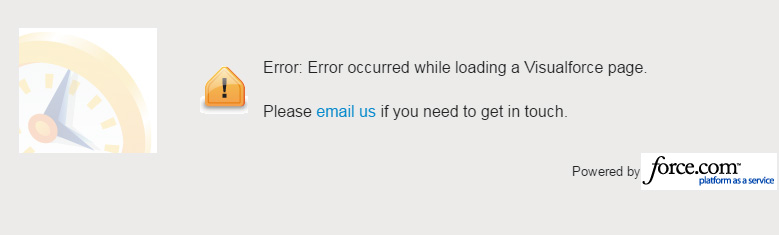
\includegraphics[width=\linewidth]{10/05_certification_error}
        \centering
        \caption{Error trobat intentant iniciar el procés de certificació}\label{fig:errorCErtification}
    \end{figure}

    Després d’una setmana sense aconseguir enviar el formulari, es va procedir a enviar un tiquet de suport mitjançant l’eina pensada per aquesta finalitat, en la plataforma per desenvolupadors. Malauradament, tampoc es va obtenir una resposta durant les següents dues setmanes.

    Finalment, al 20 d’Agost, després de buscar pel grup de desenvolupadors de FamilySearch de Google i per la pàgina de l’organització, es va aconseguir trobar un correu electrònic destinat a oferir suport als desenvolupadors. A falta d’una resposta en el tiquet de suport obert, es va decidir contactar-los per via directa tot explicant-ne el cas.

    Finalment, al cap d’un parell de dies es va rebre la resposta de què ens posarien amb contacte amb el mànager del procés de certificació i tres dies més tard, el mànager es va posar en contacte amb nosaltres per tal de ser orientat en l’ús de l’aplicació.

    Després d’un reconeixement inicial, el mànager va quedar bastant impressionat amb el MVP plantejat (\ref{fig:gordonEmail}) i també sentia curiositat per veure quins resultats es podrien obtenir amb les dades de producció. Per aquest motiu, vam decidir realitzar una vídeo conferència per veure com podíem procedir.

    \begin{figure}[h]
        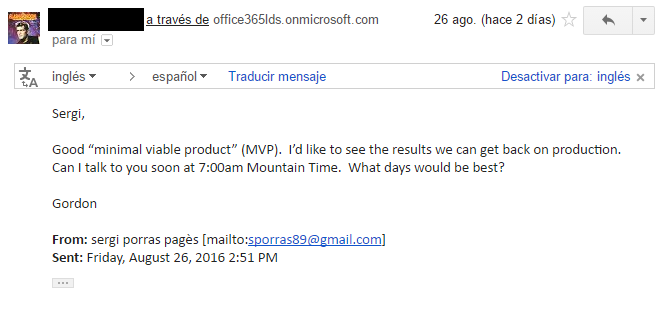
\includegraphics[width=\linewidth]{10/06_emailGordon}
        \centering
        \caption{Email del mànager de certificació de FamilySearch}\label{fig:gordonEmail}
    \end{figure}

    \paragraph{}
    Aquesta va durar al voltant d’una hora i vam ser gravats explicant, al mànager del procés de certificació, en que consistia l’aplicació i com funcionava. També anàvem responent a les diferents preguntes que el mànager pogués tenir sobre com es realitzaven les diferents interaccions amb l’API.

    Durant aquesta reunió, també vam rebre un accés a producció limitat, que consisteix en el dret d’accedir a les dades reals emmagatzemades per FamilySearch, pel grup de desenvolupadors i un màxim de fins a 100 persones externes, però en el que es demana que no es publiqui l’aplicació de forma generalitzada al públic.

    Aquest estat, serveix el propòsit d’acabar de refinar l’aplicació, mentre aquesta és certificada pels experts tècnics de l’organització FamilySearch. Es pot veure una còpia del contracte d’ús limitat que va haver de ser firmat, a l’annex B d'aquesta memòria.

    Durant aquesta reunió, l’organització també va plantejar l’opció d’alliberar el codi font del projecte, com a codi obert, amb l’objectiu de poder enllaçar-lo a la seva pàgina per desenvolupadors, conjuntament als SDK i altres eines de desenvolupament, perquè diferents persones poguessin contribuir en l’evolució del projecte.
